\documentclass[a4paper,12pt,oneside]{book}
\usepackage[utf8]{inputenc}
\usepackage[czech]{babel}
\usepackage[shellescape,latex]{gmp}
\usepackage[T1]{fontenc}
\usepackage{amsmath}
\usepackage{amssymb}
\usepackage[onehalfspacing]{setspace}
\usepackage{graphicx}
\usepackage{prettyref}
\usepackage[czech]{varioref}
\usepackage[czech,lined,boxed]{algorithm2e}
\usepackage[]{nomencl}
\usepackage{todonotes}

\setlength{\emergencystretch}{3em}

% czech prettyref
\newrefformat{eq}{\textup{(\ref{#1})}}
\newrefformat{lem}{Lemma \ref{#1}}
\newrefformat{thm}{Teorém \ref{#1}}
\newrefformat{cha}{Kapitola \ref{#1}}
\newrefformat{sec}{Sekce \ref{#1} na straně \pageref{#1}}
\newrefformat{tab}{Tabulka \ref{#1} na straně \pageref{#1}}
\newrefformat{fig}{Obrázek \ref{#1} na straně \pageref{#1}}

% B+Tree
\newcommand{\BPTree}{B$^{\text{+}}$tree}
% M-Index
\newcommand{\MIndex}{\mbox{M-Index}}

% filename
\newcommand{\filename}[1]{\texttt{#1}}

% method
\newcommand{\method}[1]{\texttt{#1}}

% type
\newcommand{\type}[1]{\texttt{#1}}

% command
\newcommand{\cmd}[1]{\texttt{#1}}

% java macros
\newcommand{\javac}{\cmd{javac}}
\newcommand{\classfile}{\filename{.class}}
\newcommand{\bytecode}{\emph{bytecode}}

\begin{document}
\frontmatter
\begin{titlepage}
\begin{center}
{\Large VYSOKÁ ŠKOLA FINANČNÍ A~SPRÁVNÍ, o.p.s.}

{\large Fakulta sociálních studií\\
Katedra informatiky\\
Bakalářské studium kombinované}
\vfill
{\Large Karel Rank\\[1in]}

{\large Implementace a srovnání výkonu implementací DB indexu v~C++, .NETu a Javě\\
Implementation and efficiency comparison of implementations of a database index in programming languages C++, .NET and Java}
\vfill
{\Large BAKALÁŘSKÁ PRÁCE}
\vfill
{\large Praha 2013}

\end{center}
{\large Vedoucí bakalářské práce: RNDr. Jakub Lokoč, Ph.D.}
\end{titlepage}
\section*{Poděkování}
Děkuji vedoucímu této práce RNDr. Jakubovi Lokočovi, Ph.D. za odborné konzultace a cenné připomínky při vedení této práce.
\newpage
\section*{Prohlášení}
Prohlašuji,

že jsem tuto závěrečnou práci vypracoval zcela samostatně a veškerou použitou literaturu a další podkladové materiály, které jsem použil, uvádím v~seznamu literatury a že svázaná a elektronická podoba práce je shodná. Současně prohlašuji, že souhlasím se zveřejněním této práce podle § 47b zákona č.~111/1998 Sb., o~vysokých školách a o~změně a doplnění dalších zákonů (zákon o~vysokých školách), ve znění pozdějších předpisů.

\bigskip
\begin{flushright}
26. dubna 2013, Karel Rank
\end{flushright}

\newpage
\section*{Abstrakt}
\section*{Abstract}
This theses aims on \MIndex{} -- a similarity search structure for multimedia databases and its implementation in Java.
The thesis contains description of \MIndex{} its structures, used algorithms and principles of metric space and similarity searching.
The implementation in Java is then measured with different sets of parameters and results are discussed together with pitfalls of micro-benchmarking code written in Java.
At the end is done performance comparison between \MIndex{} implementations in languages \CC,C\# and Java.
\newpage
\section*{Klíčová slova}
Java, M-Index, Metric Index, metrický prostor, podobnostní vyhledávání, range query, algoritmy, JVM, JIT, B+Tree
\section*{Keywords}
Java, M-Index, Metric Index, metric space, similiarity search, range query, algorithms, JVM, JIT, B+Tree
\newpage
\tableofcontents
\listoftodos
\mainmatter
\chapter{Úvod}

V~posledních několika dekádách došlo ke~změně v~potřebách vyhledávání.
Už se nepožaduje/nestačí pouze exaktní nebo přibližné vyhledání textu
v~textu. S~příchodem masivního ukládání obrázků, zvukových záznamů
a videí nelze používat \uv{klasické} postupy pro indexování a následné
vyhledávání, ale musí se používat podobnostní vyhledávání. Praktické
použití je např.~rozpoznávání řeči, rozpoznávání tváří, atd\ldots{}

Jednou z~metod pro indexování a vyhledávání v~multimediálních databázích
je \MIndex\cite{Novak:2009:MIE:1637863.1638184}\@. Autoři této
metody, která vychází z~jiné indexovací metody iDistance\cite{Jagadish:2005:IAB:1071610.1071612},
jsou David Novák a Michal Baťko z~Masarykovi univerzity Brno\@.
M-index podstatných způsobem vylepšuje výkon při vyhledávání, použitím
jiných metod rozdělení datové prostoru i samotného vyhledávání pomocí
základních metod range query a hledání K~nejbližších sousedů (KNN
search)\@.

Metrický index definuje \emph{univerzální mapovací schéma} z~obecného
metrického prostoru do reálných čísel\@. Co je nejdůležitější, toto
schéma zachovává blízkost dat, tedy mapuje podobné metrické prvky
do~blízkých čísel\@. Indexovací a vyhledávací mechanismus \MIndex
u používá množinu referenčních prvků (pivotů) a optimálně využívá všechny
známé principy pro dělení, větvení a filtrování v~metrickém prostoru\@.

Charakter mapy \MIndex u umožňuje použít dobře známé techniky jako
je \BPTree\cite{Cormen:2001:IA:580470} nebo distribuované
hašovací tabulky\@.

V~této práci detailně vysvětluji principy \MIndex u, jeho implementaci
v~jazyce Java a porovnávám výkonnost implementací \MIndex{} v~jazycích
Java, \CC{} a C\#. Předpokladem je, že na stejném stroji a na stejné
množině dat, implementace v~\CC{} zpracuje požadavky v~nejkratším
čase. Následována implementací v~C\# nebo v~Java. Podle mého názoru,
lze zrychlit běh programu v~jazyce Java tím, že se dodatečně povolí
agresivní optimalizace a \uv{zahřátím} JVM. Toto zkoumám na závěr této práce.

\section{Multimediální databáze}

Multimediální databáze je databázový systém, který umožňuje spravovat
multimediální data\@.~Multimediální data jsou nestrukturovaná data,
vyznačující se velkým objemem\@.~Typy a použití těchto databází
jsou různé, např.:


\paragraph{Autentizační Multimediální Databáze}

Skenování oční duhovky a vyhodnocování autentičnosti\@. Lze použít
i v~medicíně při diagnostikování nemocí


\paragraph{Balistická databáze}

Porovnávání otisků na nábojnicích z~místa činu a kohoutkem střelné
zbraně, např.~systém Drugfire\cite{drugfire}

\paragraph{Google Images}

Firma Google nabízí možnost vyhledávání obrázků na internetu.
Umožňuje vyhledávat podle textu spojeného s obrázkem, velikostí, barvou a atd\ldots{}
V pokročilém vyhledávání umožňuje vyhledávat obrázky podobné daného vzoru\cite{miller2011using}.

\subsection{Problémy spojené s~multimediálníma databázemi}

V~multimediální databázi narážíme na několik problémů odlišných od
,,klasických'' RDBMS, případně oproti \emph{key-value }databázím\cite{no-sql}:
\begin{itemize}
\item prokletí počtu dimenzí (\emph{curse of dimensionality})\cite{Bellman195706}
\item multimediální soubory (objekty) jsou velké
\item datové struktury jsou pro jeden typ multimédií --- zvukový záznam
má jiná kritéria než obraz
\item problém indexování takových objektů
\end{itemize}

\section{Metrický prostor}


\subsection{Předpoklady pro metrické vyhledávaní}

\emph{Metrický prostor }$\mathcal{M}$ je pár $\mathcal{M}=(\mathcal{D},d)$,
kde $\mathcal{D}$ je \emph{doména} prvků a $d$ je \emph{funkce vzdálenosti}
$d\;:\;\mathcal{D}\times\mathcal{D}\rightarrow\mathbb{R}$ splňující
následující požadavky pro všechny $o,p,q\in\mathcal{D}$:

\begin{align*}
d(o,p) & \geq0 &  & \textrm{(nezápornost)}\\
d(o,p) & =0\Longleftrightarrow o=p &  & \textrm{(identita)}\\
d(o,p) & =d(p,o) &  & \textrm{(symetrie)}\\
d(o,q) & \leq d(o,p)+d(p,q) &  & \textrm{(trojúhelníková nerovnost)}
\end{align*}



\subsection{Podobností hledávání}

Metrický prostor jako model podobnosti je typicky prohledáván podle
vzoru \emph{example-by-query} \textendash{} dotaz je vytvořen dle
\emph{prvku} $d\in D$ a daného \emph{omezení} na data, která mají
být vybrána z~indexované množiny$X\subseteq D$\@. Nejjednodušší
jsou dva typy dotazů: \emph{range~query}~$R(q,r)$\footnote{Range Query je podrobně popsán viz. \vref{sec:Range-Query}
}, který vybere všechny prvky $o\subseteq X$ ve vzdálenosti $r$~od~$q$
(např. $\left\{ o\subseteq X\mid d(q,o)\leq r\right\} $), a \emph{nearest
neighbors query} $kNN(q,k)$, který vrátí $k$~nejbližších prvků
od $q$~z~$X$\@.

\MIndex{} využívá několika struktur\@. V~následujících částí se budeme
zabývat popisem pravidel (algoritmů), které jsou zapotřebí k~utvoření
a správného používání \MIndex u.
\chapter{\MIndex{}}

V~této části je popsán a vybudován Metrický Index --- jeho principy, architektura a prohledávání.
Text a obrázky v~této kapitole jsou vlastním volným překladem nebo převzaty s~odpovídajícím označením z~původního popisu \MIndex{u}\cite{Novak:2009:MIE:1637863.1638184}.

\section{\MIndex{} prvního stupně}

Jak bylo již zmíněno, koncept \MIndex{u} je inspirován iDistance, která je indexovací metodou pro podobnostní vyhledávání ve vektorovém prostoru.
Pokud máme vzorovou množinu $S\subseteq\mathbb{\mathcal{D}}$, pak iDistance rozdělí $S$ na $n$~clusterů a utvoří referenční bod $p_{i}$ pro každý cluster $C_{i},\: i\in\left\{ 0,\ldots,n-1\right\} $.
Každému prvku $o\in X$ je pak přiřazen číselný klíč odpovídající vzdálenosti od referenčního prvku clusteru.
Pokud máme dostatečně velkou konstantu $c$ pro oddělení jednotlivých clusterů, pak iDistance klíč pro prvek
$o\in C_{i}$ je
\[
iDist(o)=d(p_{i},o)+i\cdot c
\]


Tento vzorec mapuje všechny prvky z~jakéhokoliv clusteru $C_{i}$ do intervalu $[i\cdot c,(i+1)\cdot c]$ --- viz \ref{fig:iDistance}.
Datové objekty jsou poté uloženy do \BPTree{} podle jejich \emph{iDist} klíčů.
Při prohledávání je iDistance prostor procházen podle principu -- pro \emph{range query} $R(q,r)$ můžeme určit několik intervalů
\emph{iDist} klíčů, které musejí být vyhodnoceny v~rámci dotazu.

\begin{figure}[t]
\center
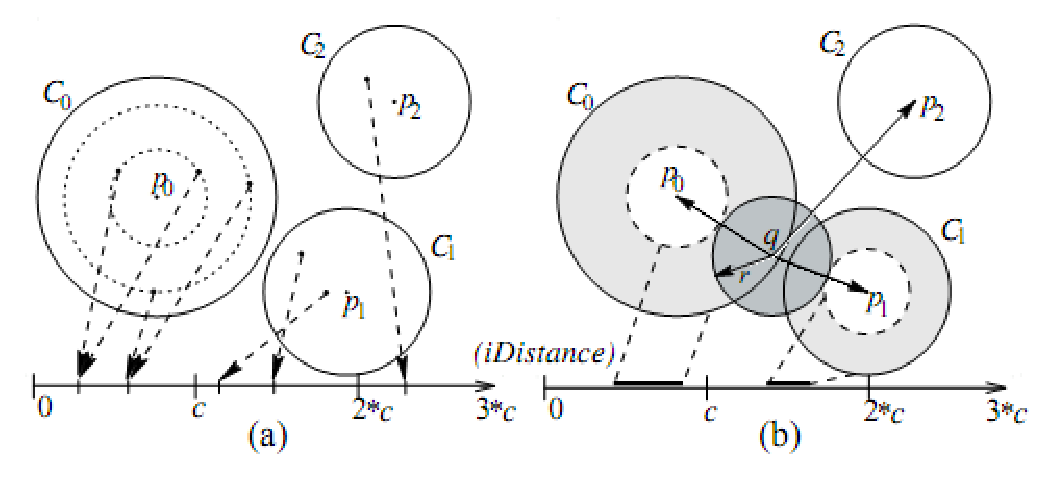
\includegraphics[clip,scale=0.4]{idistance}

\caption{iDistance}
\label{fig:iDistance}
\end{figure}

\MIndex{} zobecňuje iDistance tak, že může být použit na~obecné metrické prostory -- ne jenom na vektorový prostor.
Toho je dosaženo tím, že se vybere množina $n$~pivotů $p_{0},p_{1},\ldots,p_{n-1}$ a apriori ze vzorové množiny $S\subseteq\mathcal{D}$ a poté aplikováním Voroného dělení a rozdělení prostoru na $n$~clusterů. \prettyref{fig:M-Index-level-one} ukazuje příklad takového rozdělení ve 2D pro 4 pivoty ($n=4)$.

\begin{figure}[t]
\center
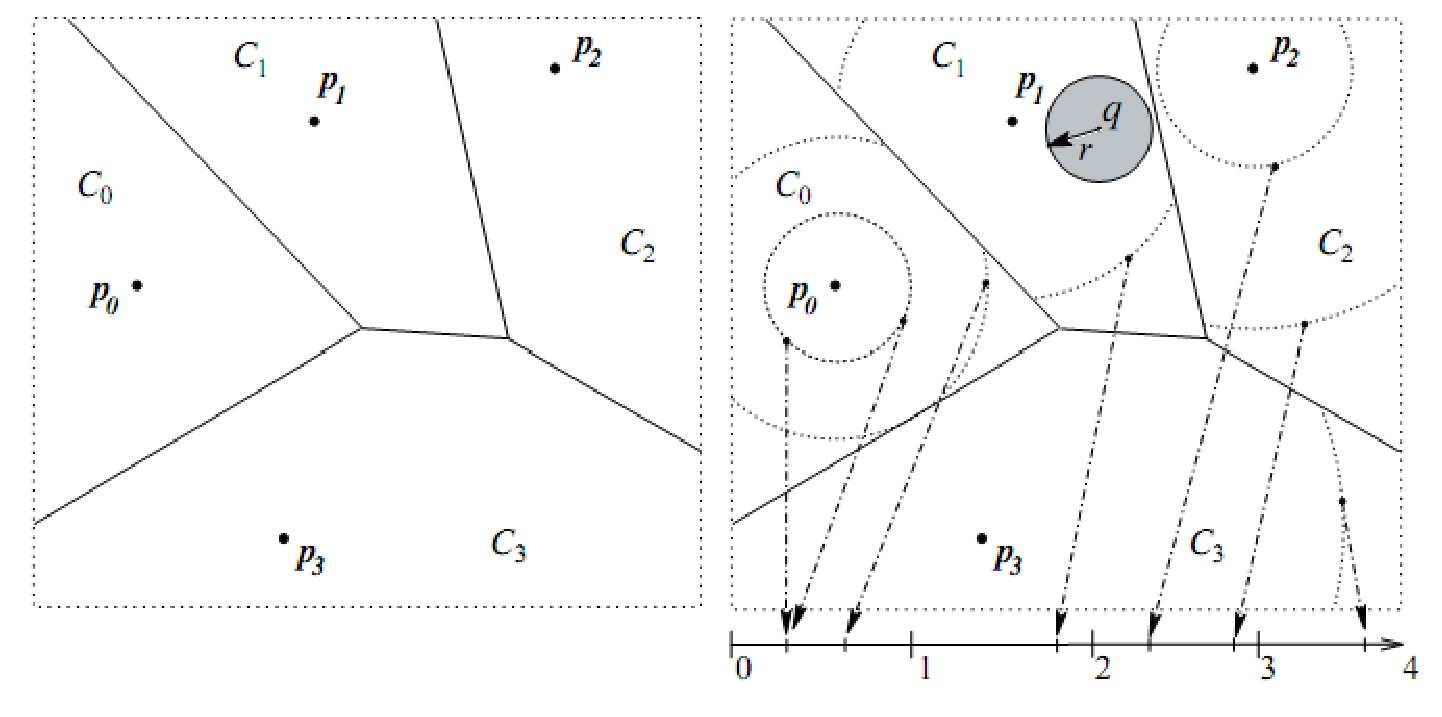
\includegraphics[scale=0.5]{m-index-level-one}
\caption{\MIndex{} prvního stupně $(l=1)$}
\label{fig:M-Index-level-one}
\end{figure}

\section{Vícestupňový \MIndex{}}

Aby byl \MIndex{} škálovatelný pro~rostoucí množství dat, budeme chtít
aplikovat další rozdělování clusterů. Pro~daný cluster $n$~pivotů
$\{p_{0},p_{1},\ldots,p_{n-1}\}$ a prvek $o\in\mathcal{D}$, platí

\[
(\cdot)_{o}\,:\,\{0,1,\ldots,n-1\}\rightarrow\{0,1,\ldots,n-1\}
\]

je permutace indexů tak, že

\[
d(p_{(0)_{o}},o)\leq d(p_{(1)_{o}},o)\leq\cdots\leq d(p_{(n-1)_{o}},o)
\]
Jinak: řada $p_{(0)_{o}},p_{(1)_{o}},\ldots,p_{(n-1)_{o}}$ je seřazena
podle vzdáleností mezi pivoty a prvkem $o$\@.

\MIndex{} s~$l$ stupni, kde $l$ je celé číslo $1\leq l\leq n$, rozděluje
prostor $\mathcal{D}$ do $n\cdot(n-1)\cdot\cdots\cdot(n-l+1)$ clusterů
za použití rekursivního Voroného dělení: Na prvním stupni je každý
prvek $o\in\mathcal{D}$ přiřazen k~jeho nejbližšímu pivotu $p_{(0)_{o}}$ --
takto se utvoří clustery $C_{i}$\@.
Na druhém stupni se každý cluster
$C_{i}$ rozdělí na $n-1$ clusterů tím samým způsobem s~použitím
$n-1$ pivotů $\{p_{1},\ldots,p_{i-1},p_{i+1},\ldots,p_{n}\}$ a vytvořením
clusterů $C_{i,j}$\@. Jinými slovy, cluster $C_{i,j}$ je tvořen
prvky $o\in X$, pro které pivot $p_{i}$ je nejbližší a $p_{j}$
je druhý nejbližší: $(0)_{o}=i$ a $(1)_{o}=j$\@.
Tento postup je zopakován $l$-krát\@.

\begin{figure}[t]
\centering{}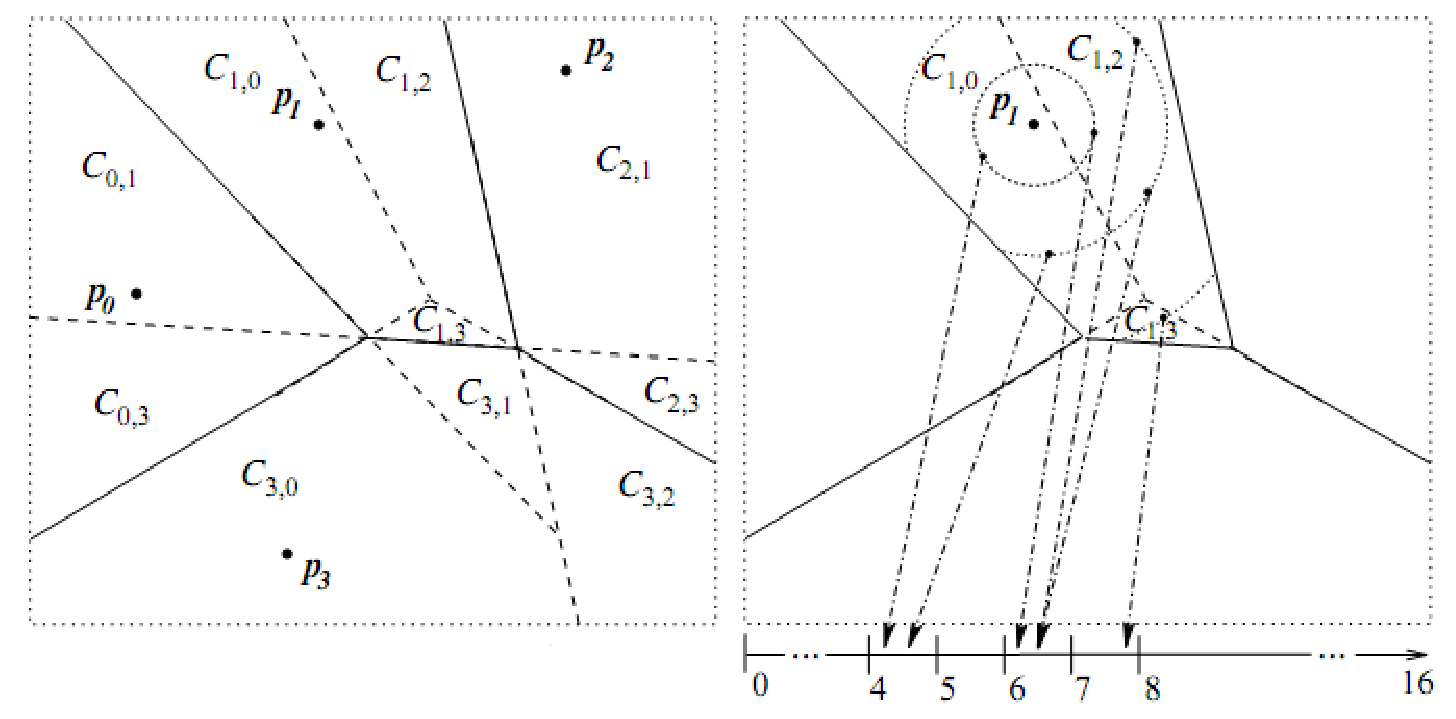
\includegraphics[scale=0.5]{m-index-level-two}\caption{\MIndex{} druhého stupně $(l=2)$}
\label{fig:M-Index-level-two}
\end{figure}


Mapovací klíč \MIndex{u} je definován $key_{l}\,:\,\mathcal{D\rightarrow\mathbb{R}}$\@.
Nechť $o\in\mathcal{D}$ patří do clusteru $C_{i_{0},i_{1},\ldots,i_{l-1}}$\@.
Celočíselná část klíče $key_{l}(o)$ identifikuje cluster: je rovna
číslu \uv{$i_{0}i_{1}\ldots i_{l-1}$'}. Desetinná část klíče $key_{l}(o)$
je vzdálenost mezi prvkem $o$ a jeho nejbližším pivotem $d(p_{(0)_{o}},o)$\@.
Celé mapování \MIndex{u} vyjádříme následujícím vztahem\cite{Novak:2009:MIE:1637863.1638184}

\begin{equation}
key_{l}=d(p_{(0)_{o}},o)+\sum_{i\text{=0}}^{l-1}(i)_{o}\cdot n{}^{(l-1-i)}\label{eq:M-Index-key}
\end{equation}


\prettyref{fig:M-Index-level-two}\cite{Novak:2009:MIE:1637863.1638184} zobrazuje mapování pro dvoustupňový
\MIndex{} $(l=2)$\@. Velikost domény je $4^{2}=16$ a prvky z~clusteru
$C_{i,j}$ jsou mapovány do intervalu $[i\cdot n+j,i\cdot n+j+1]$\@.


\section{\MIndex{} s~dynamickými stupni\label{sec:Dynamic-Cluster-Tree}}

Vícestupňový \MIndex{} zlepšuje dělící schopnosti oproti jednostupňovému \MIndex{u} seskupováním/shromažďováním blízkých prvků do menších clusterů\@.
Teoreticky, čím více stupňů \MIndex{} má, tím je vyhledávání efektivnější.
Na druhou stranu, velké množství malých clusterů vede k~větší fragmentaci dat při dotazu a větší náročnosti při provádění dotazu.
V~praxi to vede ke ztrátě výhody z~vícestupňovosti.

Koncept \MIndex{u} může být rozšířen o~dynamický počet stupňů, který umožní \prettyref{eq:M-Index-key} dynamicky zvětšovat (prohlubovat) pro velké clustery, protože \prettyref{eq:M-Index-key-max-level} požaduje pouze lokální změny klíčů \MIndex{u}
Toto vylepšení vyžaduje následující modifikace:
\begin{itemize}
\item je vybrán fixní \uv{maximální stupeň \MIndex{u}} $1\leq l_{max}\leq n$
a doména pro~tento maximální stupeň $n^{l_{max}}$ je alokována
\item rovnice \prettyref{eq:M-Index-key} pro $key_{l}$ stupně $l,\,1\leq l\leq l_{max}$
je změněna na\cite{Novak:2009:MIE:1637863.1638184}:
\begin{equation}
key_{l}=d(p_{(0)_{o}},o)+\sum_{i\text{=0}}^{l-1}(i)_{o}\cdot n{}^{(l_{max}-1-i)}\label{eq:M-Index-key-max-level}
\end{equation}

\item je vytvořen dynamický \emph{cluster tree}, který určuje aktuální hloubku
pro dané \MIndex{} clustery
\end{itemize}
Jak vypadá taková stromová struktura pro $l_{max}=3$ je zobrazeno
na~\prettyref{fig:Dynamic-Cluster-Tree}\cite{Novak:2009:MIE:1637863.1638184}. Prvky mají přiřazeny
klíče v~nejnižších patrech (listech). Typicky se nastaví limit na
možný počet prvků/dat uložených v~clusteru a zvýší se stupeň clusteru
při jeho zaplnění.

\begin{figure}[t]
\centering
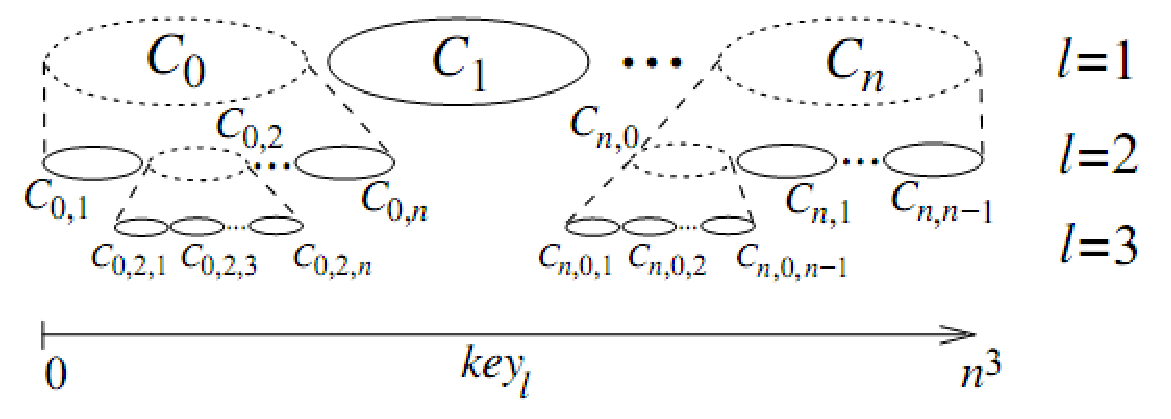
\includegraphics[scale=0.5]{m-index-dynamic-cluster}
\caption{Dynamický \MIndex{}}
\label{fig:Dynamic-Cluster-Tree}
\end{figure}

Rozdělení clusteru o~jeden stupeň znamená lokální přetřídění prvků
patřících do clusteru. Pokud zarovnáme počet pivotů~$n$ na násobky
2, pak každý stupeň $key_{l},\,1\leq l\leq l_{max}$ definuje určitý
počet bitů integrální části $key_{l_{max}}$\@. Toto přiřazení je
velmi podobné \emph{extensible hashing}\cite{Fagin:1979:EHF:320083.320092}
a rozdělení takového clusteru znamená zohlednění dalších bitů z~$key_{l_{max}}$\@.
V~praxi je $l_{max}$ limitován pouze $n$, případně rozsahem číselné
reprezentace $key$ \@.


\section{Range Query\label{sec:Range-Query}}

Zde popíšeme algoritmus \emph{range~query} $R(q,r)$ jako základní dotaz podobnosti, kde $q$ je objekt v~jehož blízkosti se má hledat a $r$ je poloměr vzdálenosti. Objekt $q$ nemusí existovat v~\MIndex{u}. 


V~prvním kroku se spočítají vzdálenosti $d(p_{i},q),\, i=1,\ldots,n$,
všech $n$~pivotů k~dotazovanému prvku (objektu)\@. Algoritmus
bere v~potaz všechny clustery na stupních $1,\ldots,l$ (pro fixní
\MIndex{} nebo projde celý strom clusterů (\emph{cluster~tree})\@.
Díky opakovanému Voroného dělení a podle \emph{Double-Pivot Distance
Constraint}\cite{similaritysearch2006}, cluster $C_{i}$ může být
vynechán, pokud
\[
d(p_{i},q)-d(p_{(0)_{q}},q)>2\cdot r
\]
kde $p_{(0)_{q}}$ je pivot nejbližší ke~$q$\@. Protože Voroného
dělení je opakováno $l$-krát pro stupeň $l$, toto pravidlo může
být opakováno $l$-krát pro cluster $C_{i_{0},\ldots,i_{l-1}}$\@.
Na každém stupni $j,\,1\leq l\leq l$ jsou pivoty $p_{i_{0},\ldots,i_{j-2}}$
ignorovány omezovacím mechanismem, protože byly vynechány Voronovým
dělením na stupni $l$\@.

Znalostí minimální a maximální vzdáleností mezi pivoty v~clusteru
(který jsou uloženy v~listech stromu), můžeme uplatnit \emph{Range Pivot
Distance Constraint}\cite{similaritysearch2006} a nemusíme přistupovat
ke clusteru $C_{p,*}$ pokud
\[
d(p,q)+r<r_{min} \quad \vee \quad d(p,q)-r>r_{max}
\]
kde $r_{min}$ a $r_{max}$ je minimální a maximální vzdálenost prvků
v~daném clusteru\@.

Pokud žádný z~výše uvedených filtrujících mechanismů neodfiltruje
cluster $C_{i_{0},\ldots,i_{l-1}}$ na úrovni listů, pak můžeme určit
interval pro $key$ domény, které mají být prohledány v~tomto clusteru:
\[
[d(p_{i_{0},}q)-r,d(p_{i_{0}},q)+r]
\]

kde oba limity jsou posunuty o~celočíselnou část klíčů clusteru $C_{i_{0},\ldots,i_{l-1}}$ podle
$key_{l}$ rovnic \prettyref{eq:M-Index-key} nebo \prettyref{eq:M-Index-key-max-level}.
Tento mechanismus je \uv{vypůjčen} \linebreak z~iDistance a je přímou aplikací
\emph{Object-Pivot Distance Constraint}\cite{similaritysearch2006}.

Počítání vzdálenosti $d$ je ve většině metrických prostorů časově náročná operace.
Snahou je proto minimalizovat její kalkulaci i za cenu uložení některých metadat k~objektům.
Ke každému prvku  $o\in X$ může být uložena vzdálenost toho objektu od pivotů $d(p_0,o),\ldots,(p_{n-1},o)$, které je nutné  spočítat během vložení prvku do \MIndex{u}.
Tyto vzdálenosti lze využít k~tzv.~\emph{Pivot Filtering}\cite{similaritysearch2006} a zamezit kalkulaci $d(q,o)$ pokud
\[
\max_{i \in \{0,\ldots,n-1\}} |d(p_i,q)-d(p_i,o)| > r.
\]

Nakonec se vzdálenost $d(q,o)$ spočítá pro všechny neodfiltrované objekty. Pokud vzdálenost mezi prvky je v~požadovaném poloměru dotazu, objekt se vrátí:
\[
d(q,o) < r.
\]
\section{Architektura \MIndex{u}}

V~předchozích sekcích byly uvedeny algoritmy a mechanismy, které
nutí k~použití různých specifických datových struktur\@. Obecně,
datové prvky mohou být uloženy v~jakékoliv struktuře, která je indexuje
podle jejich \MIndex{} klíčů. Ideální je efektivní vyhodnocování přes
intervalové dotazy -- \BPTree{}\cite{Cormen:2001:IA:580470}%
\footnote{detailní popis \BPTree{} viz \prettyref{sec:B-plus-tree}
} je typickým představitelem takovéto struktury\@.

Implementace stromu clusterů (\emph{cluster tree}) je jednoduchá\@.
Záznam pro cluster $C_{i_{0},\ldots,i_{l-1}}$ je z: $l$, pole $\left\langle i_{0},\ldots,i_{l-1}\right\rangle $
a buď ukazatelů na podstromy $\left\langle sub_{0},\ldots,sub_{n-1}\right\rangle $
v~případě vnitřního uzlu nebo $r_{min},\, r_{max}$ pro záznam listu\@.
Strom clusterů by měl být udržován v~hlavní paměti.

\chapter{Datové struktury a algoritmy}


\section{B-tree}

B-tree\cite{Cormen:2001:IA:580470} je zobecnělý binární strom s~možností
mít více jak 2 potomky. Jeho optimalizován pro čtení a zápis velkého
objemu dat, takže je se hojně používá v~databázích a souborových
systémech.

\begin{figure}[t]
\centering{}\caption{B-tree}
\end{figure}



\subsection{Definice}

B-tree $T$ je kořenový strom (s kořenem $root[T]$) s~následujícími
vlastnostmi:
\begin{enumerate}
\item Každý uzel $x$ obsahuje následující prvky:

\begin{enumerate}
\item $n[x]$ - počet klíčů uložených v~uzlu $x$,
\item $n[x]$ samotných klíčů, uložených v~neklesajícím pořadí, tedy $key_{1}[x]\leq key_{2}[x]\leq\cdots\leq key_{n[x]}[x]$,
\item $leaf[x]$ typu boolean, který je TRUE pokud $x$ je list a FALSE
pokud je $x$ interní uzel\@.
\end{enumerate}
\item Každý vnitřní uzel $x$ obsahuje $n[x]+1$ ukazatelů%
\footnote{v~případě jazyka Java \emph{referencí}%
} $c_{1}[x],c_{2}[x],\ldots,c_{n[x]+1}[x]$ na jeho potomky (\emph{children})\@.
Uzly listů nemají žádné potomky -- jejich $c_{i}$ prvky jsou nedefinovány\@.
\item Klíče $key_{i}[x]$ oddělují rozsahy klíčů uložených v~každém podstromu:
pokud $k_{i}$ je libovolný klíč uložený v~podstromu s~kořenem $c_{i}[x]$,
pak
\[
k_{1}\leq key_{1}[x]\leq k_{2}\leq key_{2}[x]\leq\cdots\leq key_{n[x]}[x]\leq k_{n[x]+1}.
\]

\item Všechny listy mají stejnou hloubku, která se nazývá výška stromu $h$\@.
\item Jsou definovány spodní a horní hranice na množství klíčů, které může
uzel obsahovat\@. Tyto hranice můžou být vyjádřeny pomocí fixního
čísla $t\geq2$ zvaného \emph{minimální stupeň} B-tree:

\begin{enumerate}
\item Každý uzel jiný než kořen musí mít aspoň $t-1$ klíčů\@. Každý interní
uzel jiný než kořen proto má aspoň $t$ potomků\@. Pokud není strom
prázdný, potom kořen má aspoň jeden klíč\@.
\item Každý uzel obsahuje nanejvýš $2t-1$ klíčů\@. Proto interní uzel
může mít nejvýše $2t$ potomků\@. Řekneme, že uzel je plný, pokud
obsahuje přesně $2t-1$ klíčů\@.
\end{enumerate}
\end{enumerate}

\subsection{Asymptotická složitost}

\begin{tabular}{|c|c|}
\hline 
Operace & Asymptotická složitost\tabularnewline
\hline 
\hline 
SEARCH & $\mathcal{O}(\log n)$\tabularnewline
\hline 
INSERT & $\mathcal{O}(\log n)$\tabularnewline
\hline 
DELETE & $\mathcal{O}(\log n)$\tabularnewline
\hline 
\end{tabular}


\subsection{Prohledávání B-tree (B-Tree-Search)}

Prohledávání B-tree je velmi podobné jako prohledávání binárního stromu\@.
Pouze místo binárního větvení v~každém uzlu, se provádí vícecestné
větvení podle počtu potomků uzlu\@.

Vstupem je ukazatel na kořenový uzel podstromu $x$ a klíč $k$, který
má být prohledán v~podstromu\@. První volání je tedy B-Tree-Search($root[T],k$).
Pokud je $k$ v~B-tree, pak vyhledávání vrátí uspořádanou dvojici
$(y,i)$, kde $y$ je ukazatel na uzel a $i$ je pozice, takže $key_{i}[y]=k$\@.
Jinak je vrácena \uv{prázdná} dvojice%
\footnote{Původně je v~\cite{Cormen:2001:IA:580470} NIL, jenže obecně vracení
NIL, NULL a 0 ukazatelů/referencí komplikuje pozdější práci s~návratovou
hodnotou metody. Robert~C.~Martin doporučuje v~ místo prázdné
reference, vracet \uv{prázdný} objekt.

V~praxi dost často dochází ke zneužívání návratové hodnoty v~podobě
NULL, jako dalšího stavu. Místo předpokladu na existující objekt,
je nutno dělat kontrolu na neexistující objekt. Jaký je rozdíl mezi
vrácením prázdné kolekce/kontejneru nebo nulového ukazatele?%
}\@.

\begin{algorithm}[t]
\SetAlgoLined
\SetKwData{EMPTYTUPLE}{EMPTY\_TUPLE}
\SetKwFunction{BTreeSearch}{B-Tree-Search}

$i \longleftarrow 1$
\While{$i \leq n[x]$ {\bf and} $k \le key_i[x]$}{
	$i \longleftarrow i+1$}
\If{$i \leq n[x]$ {\bf and} $k = key_i[x]$}{
	\Return{x, i}}
\eIf{leaf[x]}{
	\Return{\EMPTYTUPLE}}{
        \Return{\BTreeSearch{$c_i[x], k$}}}

\caption{B-Tree-Search(x,k)}
\end{algorithm}



\subsection{Operace INSERT}

Vkládání do B-tree je výrazně složitější než stejná operace pro binární
strom\@. Podobně jako u~binárního stromu, hledáme pozici listu,
kde uložíme klíč. Bohužel u~B-tree nemůžeme jednoduše vytvořit nový
uzel pro list a ten vložit, protože výsledný strom by nebyl validní
B-tree\@. Místo toho se vloží klíč už do existujícího listu\@. Protože
nelze vložit klíč do plného listu, zavedeme operaci rozdělení (\emph{split})
plného uzlu $y$ (s~$2t-1$ klíči) okolo svého \emph{mediánu klíčů}
$key_{t}[y]$ na dva uzly, každý mající $t-1$ klíčů\@. \emph{Medián
klíč} se přesune do rodiče $y$ k~identifikaci dělícího bodu mezi
dvěma novými stromy\@. Pokud je rodič $y$ také plný, musí být nejdříve
rozdělen před vložením nového klíče. Dělení plných uzlů může tedy
vypropagovat celým stromem nahoru.


\subsubsection{Rozdělení uzlu v~B-tree}

Vstupem pro proceduru B-Tree-Split-Child je neplný vnitřní uzel $x$,
index $i$ a uzel $y$, tak že $y=c_{i}[x]$ je plným potomkem $x$\@.
Procedura poté rozdělí potomka na dva a upraví $x$ tak, že má dalšího
potomka.

Složitost je $\Theta(t)$\@.

\begin{figure}[t]
\caption{Rozdělení (\emph{split}) uzlu}
\end{figure}


\begin{algorithm}[t]
\SetAlgoLined
\SetKwFunction{BTreeSplitChild}{B-Tree-Split-Child}
\SetKwFunction{AllocateNode}{Allocate-Node}
{$z \longleftarrow \AllocateNode$}
$leaf[z] \longleftarrow leaf[y]$
n[z] = t-1
for j = 1 to t-1
	do key_j[z] = key_(j+t)[y]
if not leaf[y]
	then for j = 1 to t
		do c_j[z] = c_(j+t)[y]
n[y] = t-1
for j = n[x]+1 downto i+1
	do c_(j+1)[x] = c_j[x]
c_(i+1)[x] = z
for j = n[x] downto i
	do key_(j+1)[x] = key_j[x]
key_i[x] = key_t[y]
n[x] = n[x]+1
\caption{B-Tree-Split-Child(x, i, y)}
\end{algorithm}



\subsubsection{Vložení klíčů do B-tree jedním průchodem stromem}

K~vložení klíče $k$ do B-tree $T$ o~výšce $h$ jedním průchodem
potřebujeme $O(th)=O(t\log_{t}n)$\@. B-Tree-Insert používá B-Tree-Split-Child
k~zajištění toho, že rekurse nikdy nedojde k~plnému uzlu\@.

\begin{algorithm}[t]
\begin{lstlisting}
B-Tree-Insert(T,k)
r = root[T]
if n[r] = 2t-1
	then s = AllocateNode
		root[T] = s
		leaf[s] = FALSE
		n[s] = 0
		c_1[s] = r
		B-Tree-Split-Child(s, 1, r)
		B-Tree-Insert-Nonfull(s,k)
	else B-Tree-Insert-Nonfull(r,k)
\end{lstlisting}


\caption{B-Tree-Insert}
\end{algorithm}


Procedura B-Tree-Insert-Nonfull se vnořuje podle potřeby do stromu,
v~každém okamžiku garantující, že uzel do kterého se vnořila, není
plný díky volání B-Tree-Split-Child\@.

Rekursivní procedura B-Tree-Insert-Nonfull vloží klíč $k$ do uzlu
$x$, který je předpokládán neplný v~okamžiku volání procedury\@.
Díky B-Tree-Insert a rekursivní B-Tree-Insert-Nonfull je tento předpoklad
zajištěn\@.

\begin{algorithm}[t]
\begin{lstlisting}
B-Tree-Insert-Nonfull(x,k)
i = n[x]
if leaf[x]
	then while i >= 1 and k < key_i[x]
			do key_(i+1)[x] = key_i[x]
				i = i-1
		key_(i+1)[x] = k
		n[x] = n[x]+1
	else while i >= 1 and k < key_i[x]
			do i = i-1
		i = i+1
		if n[c_i[x]] = 2t-1
			then B-Tree-Split-Child(x,i,c_i[x])
				if k > key_i[x]
					then i = i+1
		B-Tree-Insert-Nonfull(c_i[x],k)
\end{lstlisting}


\caption{B-Tree-Insert-Nonfull}
\end{algorithm}



\subsubsection{Operace DELETE}

Není nutná pro potřeby této práce a její popis je vynechána\@. Detailní
popis je možné najít v~\cite{Cormen:2001:IA:580470}\@.


\subsection{B$^{\text{+}}$-tree\label{sec:B-plus-tree}}

B$^{\text{+}}$-tree je varianta B-tree, která ukládá hodnoty až do
listů stromu. Do interních uzlů ukládá pouze informace o~klíčích
a ukazatelích na potomky. Tento typ maximalizuje větvení interních
uzlů.

Je použit v~souborových systémech, např. NTFS, Reiser FS, JFS. Dále
v~databázích PostgreSQL, MySQL, Firebird, Oracle etc\ldots{}

\begin{figure}[t]
\caption{B+-tree}
\end{figure}



\subsubsection{Asymptotická složitost}

\begin{tabular}{|c|c|}
\hline 
Operace & Asymptotická složitost\tabularnewline
\hline 
\hline 
SEARCH & $\mathcal{O}(\log n)$\tabularnewline
\hline 
INSERT & $\mathcal{O}(\log n)$\tabularnewline
\hline 
DELETE & $\mathcal{O}(\log n)$\tabularnewline
\hline 
\end{tabular}


\subsection{Voronoi rozdělení}
\chapter{\MIndex{} implementace v~jazyce Java}


\section{Jazyk Java, JVM}

Jazyk Java je silně typovaný jazyk. Tento jazyk není interpretovaný,
výsledkem překladu je \bytecode{}.\footnote{\bytecode{} jsou instrukce pro JVM. Více viz. \prettyref{sub:JIT}} Až tento \bytecode{} je interpretován v~tzv. Java Virtual Machine (JVM\nomenclature{JVM}{Java Virtual Machine}).
Díky JVM může kód přeložený na jedné platformě (ať už Windows nebo Unix a 32bit nebo 64bit) běžet na jiné. \footnote{\emph{\uv{Write once, run anywhere}}\cite{lindholm2013java}}

Hlavní klíčové vlastnosti, jak jazyka Java, JVM a JDK\nomenclature{JDK}{Java Development Kit}
jsou tyto: automatická alokace a dealokace paměti, objektovost, generika,
překlad \bytecode{} do nativních instrukcí procesoru, bohatá
knihovna tříd v~základním JDK\ldots{}

\subsection{Automatická správa paměti -- garbage collection}

V~jazyce Java neexistují ukazatele, pouze reference. V~jazycích C/\CC{}
se musí vývojář starat o~správu paměti pomocí funkcí \method{malloc},
\method{free} (jazyk C a \CC), resp. operátorů \method{new} a \method{delete}
(jazyk \CC). V~jazyce Java, resp. v~JVM \cite{lindholm2013java} tuto starost přebírá tzv. \emph{garbage
collector} (GC\nomenclature{GC}{garbage collector}), který sleduje
dosažitelnost alokovaných objektů v~paměti JVM. Pokud GC
zjistí, že objekt není dosažitelný z~jiných objektů, uvolní pamět daného objektu.
\footnote{Podobná technika/pattern je součástí \CC 11 pomocí \type{std::shared\_ptr},
kde se používá \emph{reference counting} \cite{ISO:2012:CPP}. Tato technika není použitelná v~případě cyklických referencí. Při výskytu cyklických referencí by se měl použít i \type{std::weak\_ptr}.
}

Díky automatické správě paměti je vývoj výrazně rychlejší.
Automatická správa paměti ovšem neznamená, že program je chráněn proti všem únikům paměti.\footnote{V anj. \emph{memory leaks}.}
Pokud se např. \uv{opomene} odstranit záznam z~mapy, odkazovaná instance nikdy nebude uvažována pro GC a vznikne únik paměti.

\subsubsection{Jak funguje GC}
Ve většině JVM se používá generační GC, který vychází ze dvou vypozorovaných chování:
\begin{itemize}
  \item Většina alokovaných objektů je velmi brzy nepotřebná, tzn. nejsou na ně žádná reference
  \item Jen několik starších objektů odkazuje na mladší objekty
\end{itemize}
Tyto dvě pozorování jsou známy jako \emph{slabá generační hypotéza}\cite{hunt2011java},\footnote{V anj. \emph{weak generational hypothesis}.} která platí pro většinu programů v~Java.
K~využití této hypotézy je v~JVM rozdělena \emph{halda}\footnote{V anj. \emph{heap}} na dvě fyzické části, které jsou odkazované jako generace:

\begin{figure}[h]
\centering
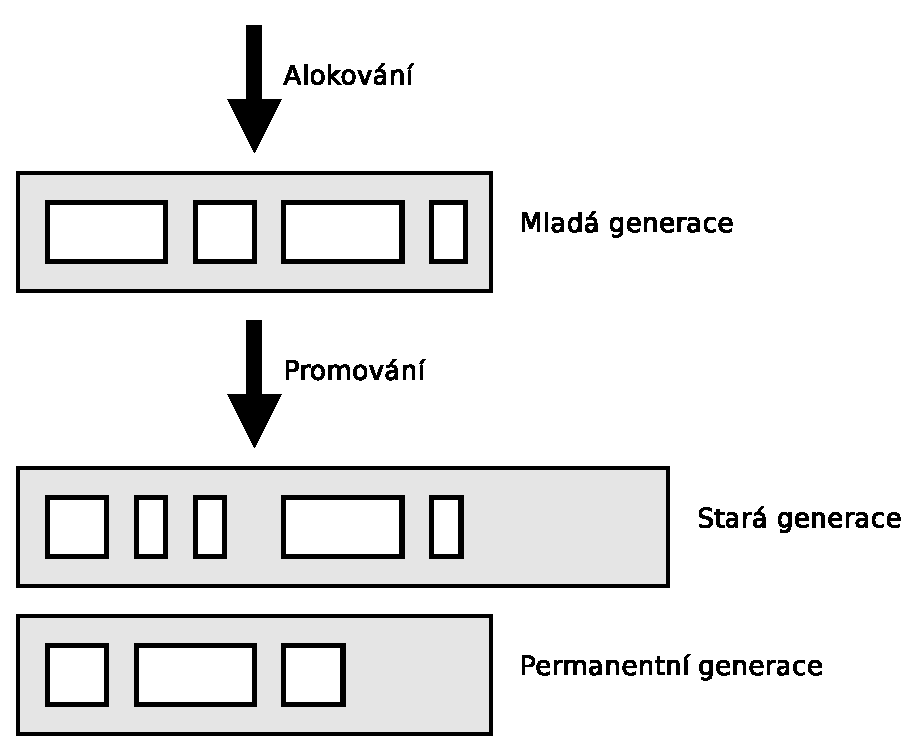
\includegraphics[width=0.5\textwidth]{jvm_memory}
\caption{Rozdělení, alokování a promování paměti v~JVM}
\label{fig:jvm_memory}
\end{figure}

\begin{description}
  \item[Mladá generace] Většina objektů je alokována do této oblasti, která je relativně malá a je často \uv{uklízena}.
Jelikož je předpoklad, že objekty jsou velmi rychle nepotřebné, jen velmi málo objektů \uv{přežije} úklid v~této oblasti.
Obecně je úklid v~této oblasti velmi efektivní, protože je prováděn v~malé oblasti paměti, která obsahuje hodně odpadních objektů.

  \item[Stará generace] Objekty, které \uv{žijí} déle, jsou promovány do této oblasti.
Tato oblast je výrazně větší než \emph{mladá generace} a její obsazování probíhá pomalu.
Úklid v~této oblasti (nazývaný \emph{full GC}) není častý, ale pokud už k~němu dojde, může být velmi dlouhý.

  \item[Permanentní generace] Toto je třetí oblastí generací, ale není použita v~generační hierarchii.
JVM ji používá pro ukládání metadat jako jsou informace o~třídách, internovaných řetězců atd\ldots
\end{description}

\subsubsection{Typy GC\label{subsub:gctypes}}

V~Oracle JVM je k~dispozici několik GC. Liší se způsobem provádění úklidu a kdy dochází k~tzv. \emph{zastavení světa}.\footnote{V anj. \emph{stop the world}}
\emph{Zastavení světa} znamená, že všechna vlákna programu jsou pozastavena a pouze vlákna pro úklid jsou v~činnosti.
Je to z~důvodu toho, aby nedocházelo k~novým alokacím objektů.
Samozřejmě, že toto má negativní dopad na aplikaci, pokud k~zastavení dochází často.

\prettyref{tab:gcs} obsahuje porovnání GC. Tabulka vyjadřuje, jakým způsobem probíhá úklid paměti jednotlivých generací.

\begin{table}
\center
\begin{tabular}{|l || l | l | p{2cm} | p{2cm} |}
\hline
& Serial GC & Parallel GC & CMS GC & G1 GC \\ \hline \hline
Paralelismus & Ne & Ano & Ano & Ano \\ \hline
Souběžnost & Ne & Ne & Ano & Ano \\ \hline
Úklid mladé gen. & Sériově & Paralelně & Paralelně & Paralelně \\ \hline
Úklid staré gen. & Sériově & Paralelně & Paralelně \& \mbox{Souběžně} & Paralelně \& \mbox{Souběžně} \\
 \hline
\end{tabular}
\caption{Porovnání GC}
\label{tab:gcs}
\end{table}

\subsection{Generika\label{sub:generika}}

Obdobně jako v~\CC{} jsou \emph{templates}\cite{ISO:2012:CPP}, jazyk Java má \emph{generics}.\footnote{Uvedeny ve verzi 1.5 \cite{gosling2013java}.}
Jsou zde rozdíly:
\begin{itemize}
  \item v~Java se informace o~typu ztrácí během překladu. Překladač nahrazuje výskyt generika za konkrétní typ (třída, rozhraní)
  \item nelze jako typový parametr použít primitivní typ -- \type{int, char, byte, long, double, float} \ldots{}
  \item nelze použít netypový parametr
\end{itemize}

Zřejmě největším přínosem je typová bezpečnost při práci s~kolekcemi a možnosti typové specializace.

\subsection{Překlad \bytecode{} do nativních instrukcí procesoru}

JVM je heap procesor. Kvůli emulaci a virtualizaci procesoru je
běh samotného \bytecode{} relativně pomalý. JVM proto překládá
za běhu \bytecode{} do nativních instrukcí procesoru, nad kterým
aktuálně JVM běží. V~JVM od Oracle
 se nazývá JIT\nomenclature{JIT}{Just In Time} Compiler\cite{hunt2011java}. Samozřejmostí je optimalizace při několika průchodech
kódem -- např. \emph{function inlining}, \emph{loop unrolling} nebo \emph{dead code elimination}\cite{hunt2011java}. Toto jsou velmi důležité vlastnosti, které mohou zásadním způsobem
ovlivnit měření výkonnosti programu. Více viz.~\prettyref{sec:vykonvjava}.

\subsection{Bohatá knihovna tříd v~základním JDK}

Java je dodávána s~rozsáhlou knihovnou JDK. Obsahuje vše nutné
pro síťovou komunikaci (RPC\nomenclature{RPC}{Remote Procedure Call}), práci s~textem -- regulární výrazy,
XML, soubory a souborový
systém a také velmi propracovanou knihovnou kontejnerů -- \emph{Java
Collections Framework }(JFC\nomenclature{JFC}{Java Collections Framework})
\footnote{V~jazyce Java se používá pro termín \emph{container} (\CC) termín
\emph{collection}}.

\section{Návrh a implementace}
Implementace \MIndex{u} je napsána pro verzi Java 7.
V~celém návrhu jsem se snažil co nejvíce používat objektově orientovaný přístup.
Tzn. že jsem se maximálně snažil omezit používaní nižších konstrukcí jazyka Java jako jsou pole a spíše využívat knihovny JDK a vyšších konstrukcí jako jsou seznamy, fronty.
Všechny implementované třídy a rozhraní jsou typově parametrizované viz. \prettyref{sub:generika}.

Při některých výpočtech bylo možné použít \emph{rozděl a panuj}\cite{Cormen:2001:IA:580470}\footnote{V anj. \emph{Divide-and-Conquer}} s~využitím \emph{Executor Framework} z~JDK.

V~popisovaných algoritmech (ať už \BPTree{} nebo \MIndex{} je často uváděna proměnná \type{leaf}, resp. zda je daná struktura list -- koncový uzel.
Z~hlediska objektového návrhu se mění chování třídy podle její datové složky, což nesvědčí o~dobrém objektovém návrhu.
K~odstranění tohoto jsem použil \emph{Replace Type Code with Subclasses}\cite{fowler1999refactoring} pro \BPTree.
V~případě \MIndex{} \emph{Range Query} jsem použil \emph{Visitor pattern}\cite{gamma1995design}.

K ověření funkčnosti jednotlivých částí kódu jsou použity \emph{unit testy} s~pokrytím více jak 70$\%$.
Nebyly pokryty jednoduché metody.
Tyto testy zabránily při změnách v~kódu regresím.

\subsection{\BPTree}
Implementace \BPTree{} se nachází v~třídě \linebreak \type{cz.rank.vsfs.btree.BPlusTreeMultiMap}. Tato mapa je typově parametrizována pro klíč a hodnotu. Protože strom musí být setříděný, musí klíč implementovat rozhraní \type{java.lang.Comparable}. Mapa umožňuje ukládat více objektů pod stejným klíčem\footnote{V \CC{} je obdobný kontejner \type{std::multimap}\cite{ISO:2012:CPP}. V~JDK žádná takováto kolekce není.} a umožňuje vyhledání v~intervalu.

Implementace mazání objektů z~mapy není potřebná pro \MIndex{} a není tudíž ani implementována.

Celý \BPTree{} je uložen v~hlavní paměti a není tedy implementováno načítaní a ukládání uzlů na disk.

\subsection{\MIndex{}}
Celá implementace \MIndex{} pracuje s~objekty, které implementují rozhraní \type{cz.rank.vsfs.mindex.Distanceable}. Tím je zajištěna případná znovupoužitelnost kódu pro jiné datové typy než je vektor.

\subsubsection{Výpočet maximální vzdálenosti mezi prvky}
Výpočet maximální vzdálenosti je NP problém, kdy se musí spočítat vzájemné vzdálenosti všech prvků v~množině a vybrat tu vzdálenost, která je největší. K~výpočtu lze použít \emph{rozděl a panuj}, takže je celý výpočet paralelní a doba výpočtu se lineárně snižuje s~počtem výpočetních vláken.

Funkcionalita je implementována ve třídě \linebreak \type{cz.rank.vsfs.mindex.MaximumDistance}.
Vzdálenost může být spočítána pouze nad objekty, které implementují rozhraní \type{Distanceable}.

Asymptotická složitost je \BigO{n^2}.

\subsubsection{Výpočet vzdáleností mezi pivoty a prvky}
K~výpočtu a seřazení vzdáleností pivotů od objektu slouží třídy implementující rozhraní \type{cz.rank.vsfs.mindex.PivotDistanceTable}. Implementovány jsou tři třídy s~tímto rozhraním.

\begin{figure}
\centering
\begin{mpost}[use,mpsettings={input metauml;}]

Interface.A("PivotDistanceTable")
	("+calculate()",
	 "+pivotAt(object:D, index:int):Pivot<D>",
	 "+firstPivotDistance(object:D):double",
	 "+distanceAt(object:D, index:int):double",
	 "+pivotDistance(object:D, pivotIndex:int):double",
);

ClassTemplate.TA("Distanceable<D>")(A);

AbstractClass.B("AbstractPivotDistanceTable")
	()();
ClassTemplate.TB("Distanceable<D>")(B);
Class.C("ParallelPivotDistanceTable")
	()();
ClassTemplate.TC("Distanceable<D>")(C);

Class.D("SimplePivotDistanceTable")
	()();
ClassTemplate.TD("Distanceable<D>")(D);

Group.g(C,D);

topToBottom.midx(30)(A,B,g);
leftToRight(80)(C,D);

drawObjects(A, B, g, TA, TB, TC, TD);
clink(realization)(B,A);
link(inheritance)(pathStepY(C.n,B.s,10));
link(inheritance)(pathStepY(D.n,B.s,10));

\end{mpost}

\caption{\type{PivotDistanceTable} UML diagram}
\end{figure}

\begin{description}
\item[ParallelPivotDistanceTable] Rozdělí úlohu na menší části podle objektů pomocí \emph{rozděl a panuj} a výpočet je paralelizován za použití všech dostupných jader systému. Tato třída je využita při konstrukci samotného \MIndex{}.
\item[SimplePivotDistanceTable] Podobně jako \type{ParallelPivotDistanceTable} vypočte vzdálenosti objektu od pivotů, ale pouze pro jeden objekt a výpočet není paralelní. Tato třída se používá v~samotném \emph{Range Query} dotazu. Pokud by se použil \type{ParallelPivotDistanceTable}, tak režije spojená s~vytvářením úloh pro exekutory, vytvořením vláken, by byla výrazně vyšší než samotný výpočet vzdáleností jednoho objektu.
\item[AbstractPivotDistanceTable] Je společným předkem obou výše uvedených tříd a obsahuje společný kód, který potomci využívají.
\end{description}

\subsubsection{Cluster tree}
\begin{figure}
\centering
\begin{mpost}[use,mpsettings={input metauml;}]

Interface.Cluster("Cluster")
	("+getIndex():Index",
	 "+accept(visitor:ClusterVisitor<D>)",
	 "+getLevel():int",
	 "+getSubCluster(pivot:Pivot<D>):Cluster<D>",
);

ClassTemplate.TCluster("Distanceable<D>")(Cluster);

Class.InternalCluster("InternalCluster")
	()();
ClassTemplate.TInternalCluster("Distanceable<D>")(InternalCluster);
Class.RootCluster("RootCluster")
	()();
ClassTemplate.TRootCluster("Distanceable<D>")(RootCluster);

Class.LeafCluster("LeafCluster")
	()();
ClassTemplate.TLeafCluster("Distanceable<D>")(LeafCluster);

Group.g(RootCluster,LeafCluster);

topToBottom.midx(30)(Cluster,InternalCluster,g);
leftToRight(80)(RootCluster,LeafCluster);

drawObjects(Cluster, InternalCluster, g, TCluster, TInternalCluster, TRootCluster, TLeafCluster);
clink(realization)(InternalCluster,Cluster);
link(inheritance)(pathStepY(RootCluster.n,InternalCluster.s,10));
link(inheritance)(pathStepY(LeafCluster.n,InternalCluster.s,10));

\end{mpost}

\caption{\type{Cluster} UML diagram}
\end{figure}

Cluster tree je tvořen třídami, které implementuji rozhraní \linebreak \type{cz.rank.vsfs.mindex.Cluster}. Jsou celkem 3 -- 
\type{InternalCluster} a jeho potomci  \type{LeafCluster} a \type{RootCluster}.

\begin{description}
\item[InternalCluster] Je použit jako vnitřní cluster. Obsahuje všechnu funkcionalitu pro udržení informací o~podstromech, objektech, informace o~minimální a maximální vzdálenosti uložené v~clusteru.
\item[LeafCluster] Reprezentuje koncový cluster. Jeho metoda \linebreak \method{LeafCluster.getSubCluster} vrací vždy konstantu \type{NO\_SUBCLUSTERS}. Toto slouží k~identifikaci koncového clusteru při utváření dynamického \MIndex{u}.
\item[RootCluster] Je použit pro kořen celého clusteru, protože vyžaduje speciální zacházení s~indexem a také při akceptování \type{ClusterVisitor}.
\end{description}

Pro změření rozdílu použití více-stupňového \MIndex{u} a \MIndex{u} s~dynamickými stupni jsou implementovány dvě třídy -- \linebreak \type{cz.rank.vsfs.mindex.MultiLevelClusterTreeBuilder} a \linebreak \type{cz.rank.vsfs.mindex.DynamicClusterTreeBuilder}. Tyto třídy jsou použity v~\type{cz.rank.vsfs.mindex.MultiLevelMIndex}, \linebreak resp. \type{cz.rank.vsfs.mindex.DynamicMIndex} ke konstrukci specifického \MIndex{u}.
Obě třídy mají téměř totožný konstruktor, pouze u~\type{DynamicClusterTreeBuilder} je navíc parametr pro maximální zaplnění koncového clusteru. Více viz \prettyref{sec:Dynamic-Cluster-Tree}.

\subsubsection{Range Query}
Díky nezávislosti dotazu na typu clusteru (více-stupňový vs. s~dynamickými stupni) je \emph{Range Query} je implementována v~třídě \type{MIndex}, která je společný rodič pro \type{MultiLevelMIndex} a \type{DynamicMIndex}. V~metodě rangeQuery není celá logika vyhledávání. V~této metodě se inicializuje ClusterRangeQuery, která implementuje samotné vyhledávání. Toto řešení jsem zvolil kvůli oddělení zodpovědnosti vyhledávání a uchovávání informací o~\MIndex{u}.\footnote{Jedná se o~tzv. \emph{Single Responsibility Principle\nomenclature{SRO}{Single Responsibility Principle}}\cite{martin2003agile}}

V~podstatě je téměř doslovně přepsán algoritmus popsaný v~\prettyref{sec:Range-Query}. Jak bylo již zmíněno v~začátku této sekce, k~odstranění nutnosti identifikování typu clusteru za běhu\footnote{V jazyce Java k~identifikaci typu slouží operátor \method{instanceof}\cite{gosling2013java}, obdobně jako v~\CC{} je operátor \method{typeid}\cite{ISO:2012:CPP}} je použit \emph{Visitor Pattern}. \prettyref{fig:rangequery-visitor-seq} popisuje toto volání detailně.


%\begin{figure}
%\centering
%\begin{sequencediagram}
%  \newthread{mi}{:MIndex}{MIndex}
%  \newinst{rq}{:ClusterRangeQuery}{}
%  \newinst{ic}{:InternalCluster}{}
%  \newinst{lc}{:LeafCluster}{}
%
%  \begin{call}{mi}{performQuery()}{rq}{nalezené objekty}
%    \begin{sdblock}{Dotaz}{dokud není fronta clusterů prázdná}
%    \end{sdblock}
%  \end{call}
%\end{sequencediagram}
%
%\caption{Sekvenční diagram volání \emph{Range Query}}\label{fig:rangequery-visitor-seq}
%\end{figure}
\missingfigure{Sekvenční volání RangeQuery}

\section{Měření výkonu v~Java\label{sec:vykonvjava}}

Abychom porozuměli úskalí měření výkonu kódu v~JVM, je nejprve nutné si přiblížit, co se děje uvnitř JVM, jak probíhá překlad a optimalizace kódu.

\subsection{Zavádění tříd}

Všechny třídy jsou přeloženy do \classfile{} souborů. Ty mohou být následně zabaleny do JAR\nomenclature{JAR}{Java ARchive}, což je v~podstatě ZIP archív. JVM při startu vyhledá tzv. Main-Class a k~ní všechny závislé třídy a k~nim další závislé třídy v~tzv. \emph{classpath}. U~každé třídy se provede statická inicializace. Toto vyhledávání není omezeno pouze na úvodní spuštění JVM. Volání \method{Class.forName()}, \method{ClassLoader.loadClass()}, \emph{Reflection API} a \method{JNI\_FindClass} může vyvolat \emph{zavádění tříd}\footnote{V anj. \emph{class loading}} kdykoliv za běhu programu, pokud požadovaná třída není již nahrána\cite{gosling2013java}\cite{lindholm2013java}.

Další fází při \emph{zavádění tříd} je i verifikace \bytecode{}. Všechny překladače Java (\javac{}) vytvářejí validní \classfile{} soubory a typově bezpečný kód. Jenže JVM se nemůže spolehnout, že soubor, který nahrála je správný. Proto musí ověřit, že je vše v~pořádku -- ať již instrukce zadané v~\classfile{} souboru nebo typová bezpečnost.

Výše popsaný proces \emph{zavádění tříd} je velmi náročný na I/O operace a zásadním způsobem ovlivní výsledek měření, pokud se nepředejde tomuto zavádění během měření.

\subsection{JIT\label{sub:JIT}}
Tradiční překladače (např. C/\CC) generují z~vyššího programovacího jazyka strojově závislý kód. Tento kód má finální podobu a všechny možné optimalizace je zapotřebí udělat během překladu. Případně použít profilování výsledné binárky a znovu nechat překladač znovu přeložit kód s~využitím profilovacích dat. Těmto překladačům se říká také statické. Výsledný kód je optimalizován pro danou platformu.

Java používá překladač \javac{}, který z~vysoko úrovňového jazyka vytvoří \classfile{}, který obsahuje \bytecode{}. JVM tento \bytecode{} následně dynamicky za běhu překládá do strojově závislého kódu pomocí JIT.

\subsubsection{Jak funguje překladač}
Každý překladač má podobnou strukturu.
Musí mít na vstupu modul pro převod zdrojového kódu do tzv. \emph{intermediate representation (IR)}\nomenclature{IR}{Intermediate Representation}.
IR je reprezentace programovacího jazyka do vnitřní formy překladače.
Existují různé typy IR. Pro každou fázi překladu se dokonce může použít jiný IR.
Všechny překladače dělají největší optimalizace právě na IR.
Množina možných optimalizací může být velmi široká a je často omezena množstvím času nutném k~provedení dané optimalizace.
Mezi jednoduché optimalizace patří zjednodušování logických výrazů, nahrazování proměnných konstantami a \emph{function inlining}.
Složitější optimalizace jsou většinou spojeny se smyčkami --\emph{loop unrolling}, odstraňování kontroly rozsahu smyčky atd\ldots{}

Když jsou tyto optimalizace hotovy, další modul vezme danou IR a převede ji do strojové podoby. Zde nastávají další optimalizace v~podobě přiřazování hodnot do registrů procesoru, výběr vhodných instrukcí atd\ldots{}

\subsubsection{Kdy JIT překládá do strojového kódu\label{subsub:whenJIT}}
JIT nepřekládá každou instrukci v~\bytecode{} ihned do strojového kódu. Většina instrukcí je na začátku interpretována. Až v~okamžiku, kdy daná instrukce se stane \emph{hot}, JIT ji zařadí pro překlad. JVM totiž udržuje u~každé metody čítač volání. Pokud daná metoda je volána více krát, stane se \emph{hot} a tím se vyvolá i její překlad. Hranice překladu je ve výchozím nastavení 10000.\footnote{Parametr pro Oracle JVM, který ovlivňuje toto nastavení je \cmd{-XX:CompileThreshold=}} Zjednodušeně řečeno: aby došlo k~překladu libovolné metody do strojového kódu, musí být daná metoda volána aspoň 10000.

Níže jsou uvedeny optimalizace, které ovlivňují výkonnost kódu.

\begin{description}
\item[function inlining] Je technika vnořování těla kódu funkcí/metod do těla volané metody. Protože každá metoda třídy je v~jazyce Java virtuální, tato optimalizace odstraňuje penalizaci za jejich volání. Ve výsledku vytváří velké bloky kódu, nad kterými se uplatňují další optimalizace. Vnořování nedochází u~všech metod. Podmínkou je, aby metoda byla krátká, což znamená, aby měla velikost do 35 \bytecode s.\footnote{V Oracle JVM lze toto omezení upravit pomocí parametru \cmd{-XX:FreqInlineSize=}} Vnořování nemůže být vynuceno. Záleží na JIT. Není ani žádné doporučení pro kompilátor jako je tomu u~\CC{} pomocí vyhrazeného slova \method{inline} u~metody.\footnote{\method{inline} říká kompilátoru, že by mohl metodu vnořit, ale záleží na chytrosti kompilátoru, zda vnoření provede\cite{Stroustrup:1997:CPL:523265}.}

Tato technika má zásadní dopad na běh programu. Ve výsledku nutí programátora navrhnout třídy tak, aby byly tvořeny malými metodami, což má za následek i dobrou čitelnost kódu.

\item[dead code elimination] JIT je schopen při analýze běhu programu identifikovat části kódu, které nemají žádný vedlejší efekt, např. pokud se výsledek volání metody nepoužije v~dalších krocích nebo. Pokud je měřící kód nesprávně navrhnut, může dojít k~tomu, že díky této optimalizaci se některé části nevykonají a výsledky měření jsou nepoužitelné.

\item[loop unrolling] Slouží k~rozbalení smyček jako je \method{for (...) ...}. Klasická optimalizace, která tělo smyčky \uv{zkopíruje} několikrát za sebou. Každá smyčka má inkrementální část a podmínku pro ukončení smyčky. Podmínka pro ukončení má vliv na \emph{branch prediction} v~CPU.\footnote{Moderní CPU mají velmi sofistikované algoritmy na předpovídání větvení programu s~předčítáním instrukcí do \emph{pipeline}. Pokud CPU špatně odhadne následující větev kódu, v~drtivé většině případů musí \uv{zahodit} a znovu načíst instrukce do \emph{pipeline}. Tato operace je velmi drahá a zastaví na několik cyklů vykonávání instrukcí CPU.} Ve výsledku se daná podmínka nevyhodnocuje tak často.

\begin{figure}
\begin{lstlisting}[frame=single,language=Java,caption=Před loop unrolling]
for (int x = 0; x < 50; x++) {
  doSomethingWith(x);
}
\end{lstlisting}
\begin{lstlisting}[frame=single,language=Java,caption=Po loop unrolling]
for (int x = 0; x < 50; x+=5) {
  doSomethingWith(x);
  doSomethingWith(x+1);
  doSomethingWith(x+2);
  doSomethingWith(x+3);
  doSomethingWith(x+4);
}
\end{lstlisting}
\end{figure}
\end{description}

\subsection{Zahřátí JVM}

Pokud bychom začali měřit jednotlivé části kódu ihned po startu JVM, neměřili bychom výkonnost samotného kódu, ale i čas za jak dlouho JVM zavede jednotlivé \classfile soubory, za jak dlouho JIT přeloží a optimalizuje instrukce \bytecode{} do strojového kódu. Pravděpodobně by se i naměřené hodnoty pro stejné testované parametry lišily, protože by k~překladu docházelo v~průběhu nebo mezi jednotlivými měřeními. Proto je nutné udělat i tzv. \emph{zahřátí JVM}.\footnote{V anj. \emph{JVM warm-up}}

Zahřátí se provádí tak, že se zavolá měřený kód tolikrát, aby se stal \emph{hot}.\footnote{Viz \prettyref{subsub:whenJIT}} Po tomto zahřátí, by již měl být měřený kód optimalizován a převeden do strojového kódu a měření by nemělo být ovlivněno.

\subsection{GC během měření}
Jak bylo uvedeno v~\prettyref{subsub:gctypes}, během úklidu paměti může dojít k~zastavení aplikace.
Je otázka, jak tomuto zastavení přistupovat při měření.
V~reálné aplikaci je toto běžné a záleží na typu aplikace, zda je zastavení celé aplikace na určitý časový okamžik problém nebo ho lze tolerovat.
Podle typu aplikace je tedy vhodné vybrat i správný \emph{garbage collector}.

V~případě testování výkonnosti určitého algoritmu je zřejmě vhodné zabránit úklidu během měření, protože ve výsledném měření bude i započítán čas nutný pro úklid paměti.
Z~aplikace je možné vynutit úklid pomocí voláni \method{System.gc()} a \uv{počkat}, dokud neproběhne úklid paměti.
V~měřeních jsem tohoto volání využil, aby se opravdu měřil čas nutný k~vykonání \emph{Range Query}.

\section{Metoda a výsledky měření}
V~měření implementace \MIndex{u} jsem se více zaměřil na praktičnost a detaily ohledně jazyka Java než na zkoumání ořezávání clusterů samotným \MIndex{em}.
Je to z~toho důvodu, že dle mého názoru původní autoři již popsali a prozkoumali principy ořezávání a jiné techniky v~rámci \MIndex{}
 
\subsection{Metoda měření\label{sec:measurementmethod}}

\MIndex{} má několik parametrů, které ovlivňují jeho chování, resp. výkonnost, v~závislosti na velikosti a typu indexovaných dat. Parametry pro měření jsou následující:
\begin{description}
\item[počet pivotů] z~kolika pivotů má být vytvořen \MIndex{}
\item[počet vyhl. objektů] kolik se má vyhledat objektů v~rámci jednoho měření
\item[max. úroveň clusteru] platí pro oba dva typy clusterů
\item[počet měření] kolik měření se má provést s~danými parametry
\item[max. počet objektů v~listech] tento parametr je pouze při měřeních dynamického clusteru a určuje maximum objektů v~listu clusteru
\item[vzdálenost] maximální vzdálenost hledaných objektů od vzorového
\item[stupeň \BPTree{}] určuje počet klíčů v~uzlech \BPTree{}. Jelikož není implementováno načítání a ukládání uzlů na disk, tento parametr ovlivňuje samotné vyhledávání ve stromu
\end{description}

Výkonnost \MIndex{u} ovlivňuje i nastavení parametrů JVM.
Zde jsem se rozhodl prozkoumat 2 parametry -- \cmd{-XX:+AggressiveOpts} a \cmd{-XX:+UseCompressedOops}, tzn. jejich vliv na výsledné měření a na jejich kombinace.

\begin{description}
\item[AggressiveOpts] Tato volba povoluje agresivní optimalizace.
Je označena jako experimentální a rozsah optimalizací se může být jiná v~každé verzi JVM.
\item[UseCompressedOops] Tato volba je dostupná pouze pro 64 bitovou verzi JVM a je vždy zapnuta, pokud není vynuceno její vypnutí při startu JVM.
V~JVM jsou všechny ukazatele na objekty schodné se strojovými ukazateli, tzn. na 64 bitové architektuře jsou 64 bitové, na 32 bitové architektuře jsou 32 bitové.
Obecně je používání 64 bitových instrukcí pomalejší oproti ekvivalentním 32 bitovým instrukcím -- vyžadují i odpovídající registry atd\ldots{}
Při zapnuté volbě \emph{UseCompressedOops} JVM komprimuje ukazatele na 32 bitů a umožňuje používat 64 bitové registry pro jiné operace, čímž snižuje penalizaci za 64 bitové instrukce.\footnote{Toto je velmi jednoduché přiblížení. Více viz \cite{hunt2011java}}
\end{description}


Průběh testu je popsán níže.

\begin{enumerate}
\item Vygenerování parametrů pro měření.
\item Načtení vstupních dat ze souboru a vytvoření vektorů.
\item Výpočet maximální vzdálenosti mezi objekty mimo třídy \type{*MIndex}, aby se pro každé nové měření nemusela znovu počítat vzdálenost.
Každá třída \type{cz.rank.vsfs.mindex.MultiLevelMIndex} a \type{cz.rank.vsfs.mindex.DynamiclMIndex} má konstruktor, který má parametr pro předpočítanou maximální vzdálenost.
\item Zahřátí JVM.
\item Opakující se test:
\begin{enumerate}
\item Vytvoření pivotů.
\item Vytvoření instance \type{\MIndex{}}.
\item Přiřazení vektorů do instance \type{\MIndex{}}.
\item Vytvoření vnitřní struktury \MIndex{u} voláním metody \method{MIndex.build()}.
\item Spuštění časovače.
\item Jednotlivé dotazy na podobnost voláním \method{MIndex.rangeQuery()}
\item Vypnutí časovače.
\item Vypsání informací o~měření -- parametry a čas vyhledávání
\item Spuštění úklidu paměti.
\end{enumerate}

Výsledné časy byly zprůměrovány.
Časovač zaznamená čas zapnutí a čas vypnutí pomocí \method{System.currentTimeInMillis()} a rozdíl je čas měření v~milisekundách.
Při tomto způsobu se nezaznamenává pouze čas vlákna, kolik taktů bylo aktivní, ale celková doba mezi zapnutím a vypnutím stopek.
Pokud je systém vytížen a měřené aplikaci se nedostává času procesoru, je měření tímto postiženo.
Měření probíhalo v~textovém režimu bez grafického prostředí, aby žádné další uživatelské procesy neovlivňovaly měření.

\end{enumerate}
\subsection{Prostředí}
Měření probíhalo v~tomto prostředí:

\begin{table}[h]
\catcode`\-=12
\center
\begin{tabular}{|l  | l | c |}
\hline
\multirow{9}{*}{CPU} & \multicolumn{2}{|c|}{AMD Phenom\texttrademark II X4 905e Processor} \\ \cline{2-3}
& Architektura & 64bit \\ \cline{2-3}
& Počet jader & 4 \\ \cline{2-3}
& Počet vláken & 4 \\ \cline{2-3}
& Frekvence & \SI{2,5}{\GHz} \\ \cline{2-3}
&  \multirow{2}{*}{L1 cache} & 4 x 64KB pro instrukce \\
& & 4 x 64KB pro data \\ \cline{2-3}
& L2 cache & 4 x 512 \\ \cline{2-3}
& L3 cache & 6MB \\ \cline{2-3}
\hline
\multirow{3}{*}{RAM} & Velikost & 12GB \\ \cline{2-3}
& Typ & DDR3 \\ \cline{2-3}
& Frekvence & \SI{1333}{\MHz} \\ \cline{2-3}
\hline
\multirow{2}{*}{Operační systém} &  \multicolumn{2}{|c|}{Debian/GNU Linux 7.0}  \\
&  \multicolumn{2}{|c|}{\tiny 3.8-trunk-amd64 \#1 SMP Debian 3.8.3-1~experimental.1 x86\_64 GNU/Linux} \\ \cline{2-3}
\hline
\multirow{2}{*}{Java} & JDK & {\tiny Java(TM) SE Runtime Environment (build 1.7.0\_13-b20)} \\ \cline{2-3}
& JVM & {\tiny Java HotSpot(TM) 64-Bit Server VM (build 23.7-b01, mixed mode)} \\ \cline{2-3}
 \hline
\end{tabular}
\caption{Informace o~stroji}
\end{table}

\subsection{Parametry měření}
\begin{table}[h]
\center
\begin{tabular}{|l|c|}
\hline
Parametr & Hodnot(a/y) \\ \hline
\hline
počet pivotů & 10, 20, 30, 50 \\ \hline
počet vyhl. objektů & 100 \\ \hline
max. úroveň clusteru & 2, 3, 4 \\ \hline
počet měření & 20 \\ \hline
max. počet objektů v~listech & 10, 20, 50, 100, 200, 300, 500 \\ \hline
vzdálenost & 0,15 \\ \hline
řád \BPTree{} & 50, 100, 500 \\ \hline
počet objektů pro porovnání & 68040 \\ \hline
dimenze objektů & 32 \\ \hline
\end{tabular}
\end{table}

Původně jsem chtěl změřit více hodnot, např. počet pivotů 100 s~max. počtem objektů v~listech 10 a úrovní clusteru 5.
Při těchto parametrech ovšem velikost clusterů byla extrémně velká -- $100 \times 99 \times 98 \times 97 \times 96 = 9034502400$.
Při práci s~tímto množstvím docházelo k~přetečení typu \type{Integer} v~kolekcích a nesmyslným výsledkům.
\footnote{V~Java je typ \type{Integer} 4 bajtový celočíselný typ se znaménkem a může mít maximálně hodnotu $2^{31}-1$}

Při tomto množství je celkový počet kombinací parametrů 252 pro dynamický cluster a 36 pro více-stupňový cluster.
Jelikož počet měření je 20 pro každý parametr, bylo celkově vykonáno 5760 měření.

Každá série měření byla spouštěna s~JVM s~různými kombinacemi parametrů, které byly uvedeny v~\prettyref{sec:measurementmethod}.
Implementace GC byla použita G1.
Pro další výklad jsem se rozhodl použít následující označení:

\begin{table}[h]
\center
\begin{tabular}{|l  || c | c |}
\hline
& AggresiveOpts & CompressedOops \\ \hline
\hline
JVM1 & Zapnuto & Zapnuto \\ \hline
JVM2 & Vypnuto & Zapnuto \\ \hline
JVM3 & Zapnuto & Vypnuto \\ \hline
JVM4 & Vypnuto & Vypnuto \\ \hline
\end{tabular}
\caption{Označení kombinací parametrů JVM}
\end{table}

\subsection{Výsledky měření}
Grafy z~měření se nacházejí jako \prettyref{ape:graphs}. Tabulkový přehled výsledků měření jsou viz \prettyref{ape:tables}.\footnote{Tabulky s~výsledky měření jsou velmi dlouhé. Nešlo jednoduchým způsobem vysázet dvě tabulky vedle sebe.}

Nejlepšího výsledku, tzn.~v~nejkratším čase, bylo dosaženo s~dynamickým \MIndex{em} s~parametry: počet pivotů 10, maximální úrovní clusteru 4, maximálním počtem objektů v~listech 10 a stupněm \BPTree{} 500.
Výsledný čas byl \SI{3485}{\ms} pro parametry JVM1.
Tato konfigurace dosáhla nejkratšího času i s~ostatními parametry JVM, pouze pro JVM2 byla až \uv{druhá}.
Rozdíl časů mezi maximálně optimalizovaným JVM a nejméně (JVM1 vs JVM4) s~těmito parametry byl více jak \SI{200}{\ms}.

Nejdelší zpracování dotazů bylo u~více-stupňového \MIndex{u} pro JVM4 s~parametry: počet pivotů 50, maximální úrovní clusteru 4 a stupněm \BPTree{} 10.
Výsledný čas \SI{5201}{\ms} a rozdíl oproti nejkratší konfiguraci je o~více jak \SI{1700}{\ms}.

\begin{figure}[h]
\centering
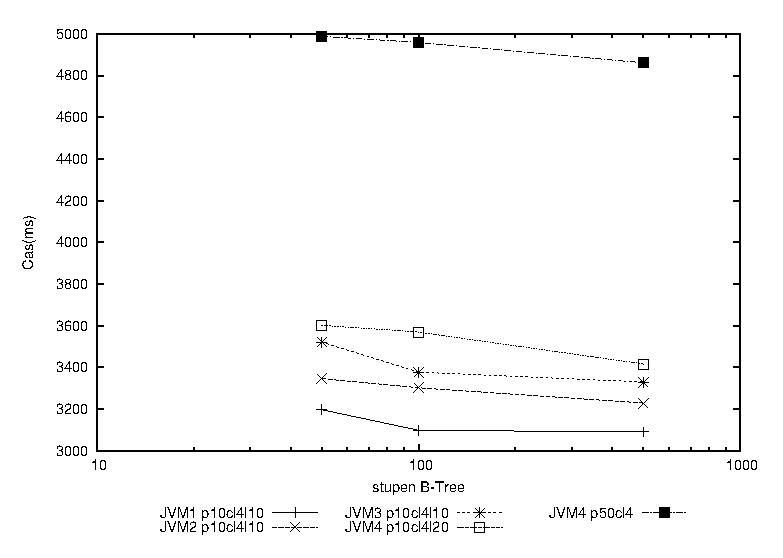
\includegraphics{best_compare}
\caption{Porovnání nejlepších a nejhorších výsledků Range Query}
\label{fig:jvm1p50}
\end{figure}

Z~výsledků měření vyplývá, že parametry JVM zásadním způsobem ovlivňují výslednou efektivitu kódu.
\prettyref{tab:jvmavgtime} zobrazuje průměrnou dobu jednoho měření.
\footnote{Hodnoty jsou spíše orientační pro posouzení vlivu parametrů JVM.}
Volba \cmd{-XX:+UseCompressedOops} je zásadní pro běh JVM v~64 bitovém prostředí.
Rozhodně není doporučeno tuto volbu vypínat.
Jak bylo uvedeno v~\prettyref{sec:measurementmethod}, volba \cmd{-XX:+AggressiveOpts} je experimentální a její efekt na výkon se může měnit mezi verzemi JVM, ale lze ji doporučit jako možný způsob zrychlení běhu programu.

\begin{table}[h]
\center
\begin{tabular}{| l  | r |}
\hline
Konfigurace JVM & Průměrný čas měření \\ \hline
\hline
JVM1 & \SI{3961}{\ms} \\ \hline
JVM2 & \SI{4205}{\ms} \\ \hline
JVM3 & \SI{4206}{\ms} \\ \hline
JVM4 & \SI{4524}{\ms} \\ \hline
\end{tabular}
\caption{Průměrný čas měření}
\label{tab:jvmavgtime}
\end{table}

Obecně konfigurace s~menším počtem pivotů (10), s~větší úrovní clusteru (4) a s~větším stupněm \BPTree{} (500) dosahovaly kratších časů.
Domnívám se, že největší vliv na výsledný čas má velikost stupně \BPTree.
Důvodem je pravděpodobně uložení klíčů v~rámci listu v~paměti, resp. CPU cache.
Vyhledání rozsahu probíhá tak, že se nalezne list stromu, který obsahuje menší klíč z~hledaného rozsahu.
V~tomto listu pak začne porovnávání klíčů, zda jsou v~požadovaném rozsahu.
Toto procházení je lineární, klíč po klíči.
Pokud se dojde na poslední uložený klíč v~listu a ten je menší než větší klíč z~hledaného rozsahu, přejde vyhledávání do sousedního listu.
Vzhledem k~tomu, že jsou klíče v~rámci listu uloženy v~paměti ve stejném paměťovém segmentu, nedochází k~častým výpadkům cache CPU.
V~případě, že je stupeň \BPTree{} menší, jsou segmenty s~klíči v~paměti více fragmentovány a dochází k~častějším výpadkům cache.
Neznamená to ovšem, že čím větší stupeň \BPTree{}, tím lépe. 
Pokud by byly uzly stromu ukládány na disk, zřejmě by byla omezena velikost stupně stromu velikostí bloku souborového systému, aby nebyl uzel stromu rozdělen do několika bloků.
Jak jsem uvedl výše, toto je má domněnka, která musí být potvrzena odpovídajícím měřením.
Jsem ale toho názoru, že toto měření je již mimo rozsah této práce.

Důvod, proč konfigurace s~nízkým počet pivotů jsou dominantní, je v~tom, že v~této množině objektů pro vyhledávání, jsou objekty shlukovány kolem konkrétních pivotů.
Režie při filtrování filtrování většího množství pivotů v~\emph{Range Query} je zřejmě signifikantní.

Je nutno podotknout, že při větší množině porovnávaných objektů (v~řádu stovek tisíců), by zřejmě \MIndex{} s~počtem pivotů 10 byl již nedostačující a neefektivně by rozděloval prostor.
Z~čehož vyplývá, že je nutné pro každou množinu objektů odladit parametry \MIndex{u} a nelze doporučit jednu konkretní konfiguraci.

\section{Srovnání výkonu implementací v~{\protect \CC}, C\# a Java}
V~této části se nachází stěžejní část práce -- samotné porovnání výkonu \MIndex{} mezi \CC, Java a C\#.

Použil jsem data, které páni Kmuníček a Koman naměřili ve svých pracích\cite{Kmunicek2011thesis}\cite{Koman2012thesis}.
Srovnání výsledných časů je nepřesné, protože jsem neměl k~dispozici stejné prostředí pro měření, v~kterém byly měřeny implementace v~\CC a C\#.
Rozdíl je především v~CPU a jeho frekvenci.
\CC a C\# byly měřeny na CPU Intel i5--430M s~frekvencí \SI{2,26}{\GHz}, Java na CPU AMD Phenom\texttrademark II X4 905e s~frekvencí \SI{2,5}{\GHz}.
Další rozdíl může být v~operačním systému a architektuře CPU (32 bit vs 64 bit).

Kolegové měřili dva dotazy o~poloměrech 0,15 a 0,25.
Vzhledem k~tomu, že jsem pro své měření používal poloměr 0,15, zvolil jsem pouze toto porovnání.
Parametry \MIndex{u} byly: maximální úroveň clusteru 3, počet pivotů 10.
Ohledně dalších parametrů měření, jsou zde určité nejasnosti:
\begin{itemize}
\item Není uvedeno, jaký stupeň byl použit pro \BPTree{}
\item Zda byl použit dynamický nebo více-úrovňový \MIndex{}
\item Časy uváděné v~obou pracích nejsou stejné. Liší se v~řádu stovek. Použil jsem časy z~\cite{Kmunicek2011thesis}.
\item Parametry kompilátoru pro kompilaci měřených programů.
\end{itemize}

Rozhodl jsem se pro porovnání použít konfiguraci s~nejlepším časem dosaženým v~Java -- dynamický \MIndex{} s~maximálním počtem 20 objektů v~listu a se stupněm \BPTree{} 500 a JVM1, a také nejhorším časem -- více-úrovňový \MIndex{} se stupněm \BPTree{} 50 a JVM4.

\begin{table}[h]
\center
\begin{tabular}{| l  | r |}
\hline
Implementace & Čas (\si{\ms}) \\ \hline
\hline
\CC & \SI{1200}{\ms} \\ \hline
C\# & \SI{6500}{\ms} \\ \hline
Java JVM1 & \SI{3500}{\ms} \\ \hline
Java JVM4 & \SI{4044}{\ms} \\ \hline
\end{tabular}
\caption{Srovnání {\protect\CC}, C\# a Java}
\end{table}

V~tomto porovnání je implementace v~Java 3-krát pomalejší s~parametry JVM1 oproti \CC.
Toto je také očekávaný výsledek.
Důvodem je zřejmě \uv{masivní používání}\cite{Kmunicek2011thesis} polí a použití pointerové aritmetiky v~implementaci \MIndex{u} v~\CC.
Implementace v~Java a C\# využívají možnosti knihoven pro daný jazyk, např. kolekcí a zaměřily se na objektově orientovaný návrh.
Používání kolekcí umožňuje rychlejší vývoj, ale v~některých případech je toto penalizováno menší výkonností výsledného kódu.
\include{proofs}
\backmatter
\nocite{*}
\begingroup
\inputencoding{latin1}
\bibliographystyle{czechiso}
\bibliography{bibliografie-bakule}
\endgroup

\printnomenclature
\listoftables
\listoffigures
\listofalgorithms

\end{document}

